%@TheDoctorRAB
%
%presentation template for class slides and research presentations
%allows for citations in slide and a list at the end
%
%%%%%
%
%REFERENCES
%
%neup.bst - numbered citations in order of appearance, short author list with et al in reference section
%nsf.bst - numbered citations in order of appearance, full author list in references section
%standard.bst - citations with author last name with et al for more than 2 authors; full author list in references section
%ans.bst is for ANS only. 
%
%author = {Lastname, Firstname and Lastname, Firstname and Lastname, Firstname} for all bst formats
%bst renders the author list itself
%
%author = {{Nuclear Regulatory Commission}} if the author is an organization, institution, etc., and not people
%
%title = {{}} for all
%
%for all - use \citep{-} - [1] or (Borrelli, 2021) in the text
%standard.bst \cite{-} - Borrelli (2021) in the text
%standard.bst lists references alphabetically
%the rest list numerically
%
%
%%% citations on slides 
%
%\citep{xxxnna} where the citation should go
%\blfootnote{\fontsize\cite{xxxnna}\fontsize\bibentry{xxxnna}} before \end{frame}
%
%
%%%%%

%%%%% presentation settings
\documentclass[aspectratio=1610,pdftex,dvipsnames,compress,xcolor={dvipsnames}]{beamer}
\usetheme{Boadilla}
\usecolortheme{seahorse}
\beamertemplatenavigationsymbolsempty
\addtobeamertemplate{footnote}{\hskip -2em}{} %pushes footnote to margin
%%% font style - can add size, etc.
%https://tug.ctan.org/macros/latex/contrib/beamer/doc/beameruserguide.pdf
\setbeamerfont{title}{series=\bfseries}
\setbeamerfont{frametitle}{series=\bfseries}
\setbeamerfont{footline}{series=\bfseries}
\setbeamerfont{author}{series=\bfseries}
\setbeamerfont{institute}{series=\bfseries}
\setbeamerfont{date}{series=\bfseries}
\setbeamertemplate{page number in head/foot}[framenumber] %just gives slide number; comment out for 1/7, 2/7...
%%%%%


%%%%% colors
%http://latexcolor.com/
%https://en.wikibooks.org/wiki/LaTeX/Colors#:~:text=black%2C%20blue%2C%20brown%2C%20cyan,be%20available%20on%20all%20systems.
%sam root
\definecolor{BackGround}{RGB}{255,250,240}
\definecolor{PrideGold}{RGB}{241,179,0}
\definecolor{Silver}{RGB}{165,169,180}
\definecolor{White}{RGB}{255,255,255}
\definecolor{Black}{RGB}{25,25,25}
\definecolor{Chrome}{RGB}{245,245,245}
%%% general
\definecolor{aliceblue}{rgb}{0.94, 0.97, 1.0}
\definecolor{antiquewhite}{rgb}{0.98, 0.92, 0.84}
\definecolor{lightmauve}{rgb}{0.86, 0.82, 1.0}
\definecolor{brilliantlavender}{rgb}{0.96, 0.73, 1.0}
\definecolor{brandeisblue}{rgb}{0.0, 0.44, 1.0}
\definecolor{darkmidnightblue}{rgb}{0.0, 0.2, 0.4}
\definecolor{darkchampagne}{rgb}{0.76, 0.7, 0.5}
%%% set slides
\setbeamercolor{background canvas}{bg=BackGround}
%%%
\setbeamercolor{block title}{bg=Silver,fg=Black}
\setbeamercolor{block body}{bg=Silver!20,fg=Black}
\setbeamercolor{block title alerted}{bg=Black,fg=Silver}
\setbeamercolor{block body alerted}{bg=PrideGold,fg=Black}
\setbeamercolor{alerted text}{fg=Silver}
\setbeamercolor*{block title example}{bg=PrideGold,fg=Black}
\setbeamercolor*{block body example}{bg=PrideGold!20,fg=Black}
%%%
\setbeamercolor*{palette primary}{bg=PrideGold,fg=Black}
\setbeamercolor*{palette secondary}{bg=PrideGold,fg=Black}
\setbeamercolor*{palette tertiary}{bg=PrideGold,fg=Black}
%%%
\setbeamercolor*{titlelike}{bg=PrideGold,fg=Black}
\setbeamercolor*{title}{bg=PrideGold,fg=Black}
\setbeamercolor*{item}{fg=PrideGold}
\setbeamercolor*{caption name}{fg=PrideGold}
%%%
\setbeamercolor*{sidebar}{fg=PrideGold,bg=Black}
\setbeamercolor*{title in sidebar}{fg=PrideGold}
\setbeamercolor*{author in sidebar}{fg=PrideGold}
\setbeamercolor*{section in sidebar}{fg=PrideGold}
%%%
\setbeamercolor{section in toc}{fg=Black}
\setbeamercolor{subsection in toc}{fg=Black}
%%%
\setbeamercolor{page number in head/foot}{fg=Black,bg=PrideGold}
%\setbeamercolor{footline}{bg=Black}
%%%
\setbeamercolor{bibliography entry author}{fg=Black}
\setbeamercolor{bibliography entry note}{fg=Black}
\setbeamercolor{bibliography entry title}{fg=Black}
%%%
\newcommand{\x}{\cellcolor{aliceblue}} %use to shade in table cell
\newcommand{\y}{\cellcolor{lightgray}} %use to shade in table cell
\newcommand{\z}{\cellcolor{antiquewhite}} %use to shade in table cell
\newcommand{\w}{\cellcolor{darkchampagne}} %use to shade in table cell

%%%%%


%%%%% general 
%\documentclass[11pt,a4paper]{article}
%\usepackage[lmargin=1in,rmargin=1in,tmargin=1in,bmargin=1in]{geometry}
\usepackage[pagewise]{lineno} %line numbering
\usepackage{setspace}
\usepackage{ulem} %strikethrough - do not \sout{\cite{}}
\usepackage{graphicx}
\usepackage{mypythonhighlight,verbatim}
\usepackage{filecontents}
\usepackage{tablefootnote}
\usepackage{footnotehyper}
\usepackage{float}
%\usepackage{subfig}
\usepackage[yyyymmdd]{datetime} %date format
\renewcommand{\dateseparator}{.}
\graphicspath{{$TEXIMG/}} %path to graphics
\setcounter{secnumdepth}{5} %set subsection to nth level
\usepackage{needspace}
\usepackage[stable,hang,flushmargin]{footmisc} %footnotes in section titles and no indent; standard.bst
\usepackage[inline]{enumitem}
\setlist[itemize]{label=\textbullet}
\usepackage{boldline}
\usepackage{makecell}
\usepackage{booktabs}
\usepackage{amssymb}
\usepackage{gensymb}
\usepackage{amsmath,nicefrac}
\usepackage{physics}
\usepackage{lscape}
\usepackage{array}
\usepackage{chngcntr}
\usepackage{hyperref}
\hypersetup{colorlinks,linkcolor=black,citecolor=black,urlcolor=blue} 
%\usepackage{sectsty}
\usepackage{textcomp}
\usepackage{lastpage}
\usepackage{xargs} %for \newcommandx
\usepackage[colorinlistoftodos,prependcaption,textsize=tiny]{todonotes} %makes colored boxes for commenting
\usepackage{soul}
\usepackage{color}
\usepackage{marginnote}
\usepackage[figure,table]{totalcount}
\usepackage[capitalise]{cleveref}
\usepackage{microtype} %improves typography for pdf
\usepackage[pdftex,dvipsnames]{colortbl} %change font color
%%%%%


%%%%% tikz
\usepackage{pgf}
\usepackage{tikz} % required for drawing custom shapes
\usetikzlibrary{shapes,arrows,automata,trees}
%%%%%


%%%%% fonts
\usepackage{times}
%\renewcommand{\sfdefault}{ubuntu}
%arial - uncomment next two lines
%\usepackage{helvet}
%\renewcommand{\familydefault}{\sfdefault}
%%%%%


%%%%% references
%\usepackage[round,semicolon]{natbib} %for (Borrelli 2021; Clooney 2019) - standard.bst 
\usepackage[numbers,sort&compress]{natbib} %for [1-3] - nsf.bst, neup.bst
\usepackage{bibentry}
\setlength{\bibsep}{7pt} %sets space between references
%\renewcommand{\bibsection}{} %suppresses large 'references' heading
%\renewcommand\bibpreamble{\vspace{\baselineskip}} %sets spacing after heading if not using default references heading
%%%%%


%%%%% tables and figures
\usepackage{longtable} %need to put label at top under caption then \\ - use spacing
\usepackage{makecell}
\usepackage{tablefootnote}
\usepackage{tabularx}
\usepackage{multirow}
\usepackage{tabto} %general tabbed spacing
\usepackage{pdfpages}
\usepackage{wrapfig} %wraps figures around text
\setlength{\intextsep}{0.00mm}
\setlength{\columnsep}{1.00mm}
\usepackage[singlelinecheck=false,labelfont=bf]{caption}
\usepackage{subcaption}
\captionsetup[table]{justification=justified,skip=5pt,labelformat={default},labelsep=period,name={Table}} %sets a space after table caption
\captionsetup[figure]{justification=justified,skip=5pt,labelformat={default},labelsep=period,name={Figure}} %sets space above caption, 'figure' format
\captionsetup[wrapfigure]{justification=centering,aboveskip=0pt,belowskip=0pt,labelformat={default},labelsep=period,name={Fig.}} %sets space above caption, 'figure' format
\captionsetup[wraptable]{justification=centering,aboveskip=0pt,belowskip=0pt,labelformat={default},labelsep=period,name={Table}} %sets space above caption, 'figure' format
%%%%%


%%%%% watermark
%\usepackage[firstpage,vpos=0.63\paperheight]{draftwatermark}
%\SetWatermarkText{\shortstack{DRAFT\\do not distribute}}
%\SetWatermarkScale{0.20}
%%%%%


%%%%% cross referencing files
%\usepackage{xr} %for revisions - will cross reference from one file to here
%\externaldocument{/path/to/auxfilename} %aux file needed
%%%%%


%%%%% toc and glossaries
\usepackage[toc,title]{appendix}
\usepackage[acronym,nomain,nonumberlist]{glossaries}
%\makenoidxglossaries
%\usepackage{titlesec,titletoc}
%\renewcommand{\thepart}{ARTICLE \Roman{part}} %puts the label into the command so \thelabel will carry through
%\renewcommand{\thesection}{\arabic{section}} %puts the label into the command so \thelabel will carry through
%\titleformat{\part}{\normalfont\large\bfseries}{\thepart}{}{}[]
%\titlespacing*\part{0pt}{0.95\baselineskip}{0.75\baselineskip}
%\titleformat{\section}[runin]{\normalfont\large\bfseries}{\thesection}{-1em}{}[.]
%\titlespacing*\section{0pt}{0.65\baselineskip}{0.55\baselineskip}
%\titleformat{\subsection}[runin]{\normalfont\normalsize\bfseries}{\thesubsection}{-1em}{}[.]
%\titlespacing*\subsection{0pt}{0.50\baselineskip}{0.35\baselineskip}
%\titleformat{\paragraph}[runin]{\normalfont\normalsize\bfseries\itshape}{\theparagraph}{-1em}{}[.]
%\titlespacing*\paragraph{0pt}{0.45\baselineskip}{0.25\baselineskip}
%\titleformat{\subparagraph}[runin]{\normalfont\normalsize\itshape}{\thesubparagraph}{-1em}{}[.]
%\titlespacing*\subparagraph{0pt}{0.40\baselineskip}{0.25\baselineskip}
%\titleformat{\paragraph}[hang]{\normalfont\normalsize\bfseries}{\theparagraph}{5pt}{}[]
%\titlespacing*\paragraph{0pt}{0.50\baselineskip}{0.25\baselineskip}
%\titleformat{\subparagraph}[runin]{\normalfont\normalsize\itshape}{\thesubparagraph}{-1em}{}[.]
%\titlespacing*\subparagraph{0pt}{0.40\baselineskip}{0.20\baselineskip}
%%%%%


%%%%% editing
\newcommand{\edit}[1]{\textcolor{blue}{#1}} %shortcut for changing font color on revised text
\newcommand{\fn}[1]{\footnote{#1}} %shortcut for footnote tag
\newcommand*\sq{\mathbin{\vcenter{\hbox{\rule{.3ex}{.3ex}}}}} %makes a small square as a separator $\sq$
%\newcommand{\sk}[1]{\sout{#1}} %shortcut for default strikethrough - do not sk through citep
\newcommand\sk{\bgroup\markoverwith{\textcolor{red}{\rule[0.5ex]{1pt}{1pt}}}\ULon} %strikethrough with red line; not in \section{}
%\st{} does strikethrough using soul package but does not like acronyms
\newcommand{\blucell}{\cellcolor{aliceblue}} %use to shade in table cell
\newcommand{\grycekk}{\cellcolor{lightgray}} %use to shade in table cell
\newcommand{\whicell}{\cellcolor{antiquewhite}} %use to shade in table cell
%%%%%


%%%%% acronyms
\newcommand{\acf}{\acrfull} %full acronym
\newcommand{\acl}{\acrlong} %long acronym
\newcommand{\acs}{\acrshort} %short acronym

\newcommand{\acfp}{\acrfullpl} %full acronym plural
\newcommand{\aclp}{\acrlongpl} %long acronym plural
\newcommand{\acsp}{\acrshortpl} %short acronym plural
%%%%%


%%%%% todonotes
\newcommandx{\cmt}[2][1=]{\todo[author=\textbf{STRUCTURE},tickmarkheight=0.15cm,linecolor=red,backgroundcolor=red!25,bordercolor=black,#1]{#2}}
\newcommandx{\con}[2][1=]{\todo[author=\textbf{CONTENT},tickmarkheight=0.15cm,linecolor=brilliantlavender,backgroundcolor=brilliantlavender,bordercolor=black,#1]{#2}}
%\newcommandx{\rab}[2][1=]{\todo[noline,author=\textbf{RAB},backgroundcolor=Plum!25,bordercolor=black,#1]{#2}}
%%%
%\newcommandx{\jon}[2][1=]{\todo[noline,author=\textbf{ATTN: Johnson},backgroundcolor=blue!25,bordercolor=black,#1]{#2}}
%\newcommandx{\han}[2][1=]{\todo[noline,author=\textbf{ATTN: Haney},backgroundcolor=OliveGreen!25,bordercolor=black,#1]{#2}}
\newcommandx{\rab}[2][1=]{\todo[author=\textbf{Borrelli},tickmarkheight=0.15cm,linecolor=black,backgroundcolor=Plum!25,bordercolor=black,#1]{#2}}
%\newcommandx{\han}[2][1=]{\todo[author=\textbf{ATTN: Haney},tickmarkheight=0.15cm,linecolor=OliveGreen,backgroundcolor=OliveGreen!25,bordercolor=OliveGreen,#1]{#2}}
%\newcommandx{\jon}[2][1=]{\todo[author=\textbf{ATTN: Johnson},tickmarkheight=0.15cm,linecolor=blue,backgroundcolor=blue!25,bordercolor=blue,#1]{#2}}
%%% highlighting 
\DeclareRobustCommand{\hlc}[1]{{\sethlcolor{LimeGreen}\hl{#1}}}
\makeatletter
    \if@todonotes@disabled
    \newcommand{\hlh}[2]{#1}
    \else
    \newcommand{\hlh}[2]{\han{#2}\hlc{#1}}
    \fi
    \makeatother

\DeclareRobustCommand{\hld}[1]{{\sethlcolor{CornflowerBlue}\hl{#1}}}
\makeatletter
    \if@todonotes@disabled
    \newcommand{\hlj}[2]{#1}
    \else
    \newcommand{\hlj}[2]{\jon{#2}\hld{#1}}
    \fi
    \makeatother

\DeclareRobustCommand{\hlf}[1]{{\sethlcolor{lightmauve}\hl{#1}}}
\makeatletter
    \if@todonotes@disabled
    \newcommand{\hlb}[2]{#1}
    \else
    \newcommand{\hlb}[2]{\rab{#2}\hlf{#1}}
    \fi
    \makeatother
%%%%%


%%%%% table alignments
\newcolumntype{L}[1]{>{\raggedright\let\newline\\\arraybackslash\hspace{0pt}}m{#1}} %uses \raggedright with m,p{} in table column
\newcolumntype{C}[1]{>{\centering\let\newline\\\arraybackslash\hspace{0pt}}m{#1}} %uses \raggedright with m,p{} in table column
\newcolumntype{R}[1]{>{\raggedleft\let\newline\\\arraybackslash\hspace{0pt}}m{#1}} %uses \raggedright with m,p{} in table column
%%%%%


%%%%% table contents
\makeatletter
\renewcommand\tableofcontents{%
    \@starttoc{toc}%
}
\makeatother

\makeatletter
\renewcommand\listoffigures{%
    \@starttoc{lof}%
}
\makeatother

\makeatletter
\renewcommand\listoftables{%
    \@starttoc{lot}%
}
\makeatother

\makeatletter
\newcommand*\ftp{\fontsize{16.5}{17.5}\selectfont}
\makeatother
%%%%%


%%%%% user commands
\newcommand\blfootnote[1]{%
  \begingroup
  \renewcommand\thefootnote{}\footnote{#1}%
  \addtocounter{footnote}{-1}%
  \endgroup
}


\makeatletter
\renewcommand{\@biblabel}[1]{#1.\hfill} %bibliography ordered list has numbers left flush
\makeatother


\AtBeginSection[]{
    \begin{frame}[plain]{}
         
         \vfill

         \centering
         \begin{beamercolorbox}[sep=8pt,center,shadow=true,rounded=true]{titlelike}
             \usebeamerfont{title}\insertsectionhead\par
         \end{beamercolorbox}

         \vfill

     \end{frame}
 }
%%%%%


%%%%% header and footer
%\usepackage{fancyhdr}
%\pagestyle{fancy}
%\fancyhf{} %move page number to bottom right
%\renewcommand{\headrulewidth}{0pt} %set line thickness in header; uncomment as is to remove line
%\lhead{\scriptsize Name}
%\lhead{\scriptsize PNUCENE-D-22-xxxxx}
%\chead{\scriptsize \textit{PhD White Paper Project Proposal}}
%\rhead{\scriptsize \today}
%\rfoot{\thepage}
%%%%%


%%%%% acronyms
\input{$ACRONYM/acronyms}
%%%%%

%%%%% spacing
%\onehalfspacing %linespacing
%\setstretch{1.05} %linespacing
%\spacing{1.25} %equivalent to 1.5 line spacing in Word
%%%%%


%%%%% linenumbering
%\linenumbers %toggle line numbers
%\pagewiselinenumbers %reset line numbers on new page
%\modulolinenumbers[1] %line numbering interval
%%%%%


%%%%% title page
\addtocounter{framenumber}{-1} %does not count the title slide in the slide count
\title[NE585 - Nuclear fuel cycles]{NE585\\NUCLEAR FUEL CYCLES\\Monte Carlo methods \& \acs{mcp} \\5 }
\author[@TheDoctorRAB]{R. A. Borrelli}
\institute[]{
    \acl{ui}\\
    \vspace{0.10in}
    
\includegraphics[width=0.20\textwidth]{logo/university-of-idaho/nuclear-engineering/ne-logo.png}
    }
\date{\acl{iff}}
%%%%%


\begin{document}


%%%%% title page with no footer
{
    \setbeamertemplate{footline}{}
    \begin{frame}
        \titlepage
    \end{frame}
}
%%%%%


\begin{frame}{Learning objectives}
    \begin{enumerate}[series=outerlist,topsep=0pt,itemsep=21pt,leftmargin=*,label=(\arabic*)]
        \item[]Modeling of nuclear systems
        \item[]Demonstrating skill with with \acs{mcp}
        \item[]Developing input files
        \item[]Interpreting output
        \item[]Lots of content on the \href{https://uidaho.pressbooks.pub/nuclearengineering/chapter/mcnp/}{\acs{oer}}
    \end{enumerate}
\end{frame}


\begin{frame}{Learning nodes}
    \begin{columns}[t]

        \begin{column}{0.50\textwidth}
            \begin{enumerate}[series=outerlist,topsep=0pt,itemsep=1pt,leftmargin=*,label=(\arabic*)]
                \item[]\textbf{Monte Carlo theory}
                \item[]Approximating an integral  
                \item[]Computing $\pi$
                \item[]Multidimensional integration
                \item[]Random sampling
                \item[]Boltzmann transport equation
                    \vspace{0.15in}
                \item[]\textbf{Solution procedure}
                \item[]Assumptions
                \item[]Superposition
                    \vspace{0.15in}
                \item[]\textbf{Random numbers}
            \end{enumerate}
        \end{column}

        \begin{column}{0.50\textwidth}
            \begin{enumerate}[series=outerlist,topsep=0pt,itemsep=1pt,leftmargin=*,label=(\arabic*)]
                \item[]\hfill\textbf{\acs{mcp} modeling}
                \item[]\hfill What it does
                \item[]\hfill Particle tracking
                \item[]\hfill Tally
                \item[]\hfill Input decks
                \item[]\hfill Geometry
                \item[]\hfill Neutron flux example
                \item[]\hfill Surfaces
                \item[]\hfill Sense
                \item[]\hfill Cells
                \item[]\hfill Universes
                    \vspace{0.15in}
                \item[]\hfill\textbf{Other tips}
                    \vspace{0.15in}
                \item[]\hfill\textbf{Additional information}
            \end{enumerate}
        \end{column}

    \end{columns}
\end{frame}


\begin{frame}[t]{More learning nodes}
    \begin{columns}[t]

        \begin{column}{0.50\textwidth}
            \begin{enumerate}[series=outerlist,topsep=0pt,itemsep=1pt,leftmargin=*,label=(\arabic*)]
                \item[]\textbf{\acs{mcp} quality control}
                \item[]Mean \& variance
                \item[]Other statistical checks
                    \vspace{0.15in}
                \item[]\textbf{Criticality}
                    \vspace{0.15in}
                \item[]\textbf{Variance reduction}
            \end{enumerate}
        \end{column}

        \begin{column}{0.50\textwidth}
        \end{column}

    \end{columns}
\end{frame}


\section{Monte Carlo theory}


\addtocounter{framenumber}{-1} 
\begin{frame}{Monte Carlo simulates particle transport}
    \begin{enumerate}[series=outerlist,topsep=0pt,itemsep=21pt,leftmargin=*,label=(\arabic*)]
        \item[]Particles like neutrons, but photons too
        \item[]Because we're engineers we are going to focus more on application than theory
        \item[]There are a lot of Monte Carlo codes (OpenMC)
        \item[]We will use the latest version of \acs{mcp}
    \end{enumerate}
\end{frame}


\section{Fundamentals of Monte Carlo particle transport\\Forrest B. Brown}
\section{\href{https://mcnp.lanl.gov/pdf_files/TechReport_2005_LANL_LA-UR-05-4983_Brown.pdf}{LA-UR-05-4983}}


\addtocounter{framenumber}{-2} 
\begin{frame}{Monte Carlo was invented by von Neumann}
    \begin{enumerate}[series=outerlist,topsep=0pt,itemsep=21pt,leftmargin=*,label=(\arabic*)]
        \item[]Fairly successful guy
        \item[]Basically invented what we call `scientific computing'
        \item[]Monte Carlo is highly accurate but expensive computationally
        \item[]\acs{mcp} can be run on just about all architectures but use linux
    \end{enumerate}
\end{frame}


\begin{frame}{Monte Carlo methods solve the transport equation}
    \begin{enumerate}[series=outerlist,topsep=0pt,itemsep=21pt,leftmargin=*,label=(\arabic*)]
        \item[]Mathematical approach is for importance sampling, convergence, variance reduction, random sampling techniques, eigenvalue calculation schemes
        \item[]Simulation approach is for collision physics, tracking, tallying
        \item[]Monte Carlo methods solve integral problems, so consider the integral form of the Boltzmann equation
        \item[]Most theory on Monte Carlo deals with fixed-source problems
        \item[]Eigenvalue problems are needed for criticality and reactor physics calculations
        \item[]Should know basic statistics
    \end{enumerate}
\end{frame}


\section{Approximating an integral}


\addtocounter{framenumber}{-1} 
\begin{frame}{Monte Carlo approximates the area under a curve}
    \begin{equation}
        \LARGE
        G = \int_0^1 g(x)dx
    \end{equation}

    \begin{equation}
        \LARGE
        g(x) = \sqrt{1-x^2}
    \end{equation}

    \vspace*{\fill}

    \begin{enumerate}[series=outerlist,topsep=0pt,itemsep=21pt,leftmargin=*,label=(\arabic*)]
        \item[]May not always be able to compute the integral
    \end{enumerate}

    \vspace*{\fill}

    \begin{equation}
        \LARGE
        G \approx \frac{1}{N} \sum_{k=1}^{N} \sqrt{1-x_k^2}
    \end{equation}

    \vspace*{\fill}

    \begin{enumerate}[series=outerlist,topsep=0pt,itemsep=21pt,leftmargin=*,label=(\arabic*)]
        \item[]Choose randomly -- $x \in (0,1)$
    \end{enumerate}
\end{frame}


\begin{frame}{Monte Carlo approximates the area under a curve}
    \begin{enumerate}[series=outerlist,topsep=0pt,itemsep=21pt,leftmargin=*,label=(\arabic*)]
        \item[]Or --
    \end{enumerate}

    \vspace*{\fill}

    \begin{equation}
        \LARGE
        x_k^2+y_k^2 \leq 1, k = 1,..,N
    \end{equation}

    \vspace*{\fill}

    \begin{enumerate}[series=outerlist,topsep=0pt,itemsep=11pt,leftmargin=*,label=(\arabic*)]
        \item[]Sample x and y and count a 'hit' if less than 1
    \end{enumerate}

    \vspace*{\fill}

    \begin{equation}
        \LARGE
        G \approx (1 \cdot 1)\frac{hits}{N}
    \end{equation}
\end{frame}


\begin{frame}{Analytical solution can be obtained here}
    \begin{columns}[t]

        \begin{column}{0.55\textwidth}
            \begin{equation}
                \LARGE
                G = \frac{1}{2}(x\sqrt{1-x^2}-sin^{-1} x)
            \end{equation}

            \vspace*{\fill}
            
            \begin{enumerate}[series=outerlist,topsep=0pt,itemsep=21pt,leftmargin=*,label=(\arabic*)]
                \item[]So the Monte Carlo routine can be checked
                \item[]Code on \href{https://github.com/TheDoctorRAB/education/blob/master/src/monte.carlo.simple.py}{GitHub}
                \item[]See also Brown 1-6
            \end{enumerate}
        \end{column}

        \begin{column}{0.45\textwidth}
            \begin{figure}
                \centering
                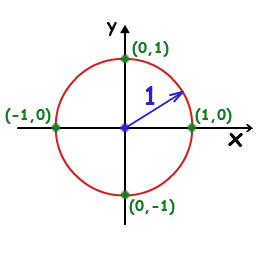
\includegraphics[width=0.85\textwidth]{ne585/circle.png}
%                \caption{}
            \end{figure}
        \end{column}

    \end{columns}
\end{frame}


\section{Computing $\pi$}


\addtocounter{framenumber}{-1} 
\begin{frame}{Use Monte Carlo to compute $\pi$}
    \begin{equation}
        \LARGE
        x^2 + y^2 = r^2
    \end{equation}

    \begin{equation}
        \LARGE
        A = \pi r^2
    \end{equation}

    \vspace*{\fill}

    \begin{enumerate}[series=outerlist,topsep=0pt,itemsep=11pt,leftmargin=*,label=(\arabic*)]
        \item[]Sample $x \in (0,r)$
        \item[]Sample $y \in (0,r)$
        \item[]That is the first quadrant of the circle
        \item[]Record hits
        \item[]Divide hits by sample number like before
        \item[]\Large $\therefore \pi \approx 4 \cdot \frac{hits}{N}$
    \end{enumerate}
\end{frame}


\section{Multidimensional integration}


\addtocounter{framenumber}{-1} 
\begin{frame}{Monte Carlo is good for multidimensional integration}
    \begin{enumerate}[series=outerlist,topsep=0pt,itemsep=21pt,leftmargin=*,label=(\arabic*)]
        \item[]The procedure is the same
    \end{enumerate}

    \vspace*{\fill}

    \begin{equation}
        \LARGE
        G = \int_{a_1}^{b_1} \ldots \int_{a_n}^{b_n} g(r_1, \ldots ,r_n) dr_1 \ldots dr_n
    \end{equation}

    \begin{equation}
        \LARGE
        G \approx (b_1-a_1) \ldots (b_n-a_n) \frac{1}{N} \sum_{k=1}^N g(r_1^k, \ldots ,r_n^k)
    \end{equation}

    \begin{equation}
        \LARGE
        r_n^k \in (a_n,b_n)
    \end{equation}
\end{frame}


\section{Random sampling}


\addtocounter{framenumber}{-1} 
\begin{frame}{The key to Monte Carlo methods is the notion of random sampling}
    \begin{enumerate}[series=outerlist,topsep=0pt,itemsep=21pt,leftmargin=*,label=(\arabic*)]
        \item[]For a given pdf $p(x)$ produce actual $Xs$ distributed in the same way
        \item[]Models the outcome of physical events
        \item[]Neutron scatting, absorption, fission
        \item[]1-8 -- 1-10
    \end{enumerate}
\end{frame}


\section{Boltzmann transport equation}


\addtocounter{framenumber}{-1} 
\begin{frame}{Monte Carlo is used to simulate the transport equation}
    \begin{equation}
        \Large
        \Psi(\underline{r},\underline{v}) = \int[\int\Psi(\underline{r}', \underline{v}') C(\underline{v}'\rightarrow\underline{v}) d\underline{v}' + Q(\underline{r}',\underline{v})] T(\underline{r}'\rightarrow\underline{r}) d\underline{r}
    \end{equation}

    \vspace*{\fill}

    \begin{enumerate}[series=outerlist,topsep=0pt,itemsep=21pt,leftmargin=*,label=(\arabic*)]
        \item[]$\Psi(\underline{r}, \underline{v})$ -- particle collision density
        \item[]$Q(\underline{r}', \underline{v})$ -- source term
        \item[]$C(\underline{v}' \rightarrow \underline{v})$ -- collision; change velocity at fixed position
        \item[]$T(\underline{r}' \rightarrow \underline{r})$ -- transport; change position at fixed velocity
    \end{enumerate}
\end{frame}


\begin{frame}{The source term can become exceedingly complex}
    \begin{enumerate}[series=outerlist,topsep=0pt,itemsep=21pt,leftmargin=*,label=(\arabic*)]
        \item[]$Q(\underline{r},\underline{v}) = S(\underline{r},\underline{v})$ -- fixed source
        \item[]$Q(\underline{r},\underline{v})= S(\underline{r},\underline{v}) + \int \Psi(\underline{r},\underline{v}') F(\underline{v}' \rightarrow \underline{v},\underline{r}) d\underline{v}'$ -- fixed source + fission
        \item[]$Q(\underline{r},\underline{v}) = \frac{1}{k} \int \Psi(\underline{r},\underline{v}') F(\underline{v}' \rightarrow \underline{v},\underline{r}) d\underline{v}'$ -- eigenvalue
    \end{enumerate}
\end{frame}


\section{Solution procedure}


\addtocounter{framenumber}{-1} 
\begin{frame}{Start with some assumptions}
    \begin{enumerate}[series=outerlist,topsep=0pt,itemsep=21pt,leftmargin=*,label=(\arabic*)]
        \item[]Static, homogeneous medium
        \item[]Time independent
        \item[]Markovian (important)
        \item[]Neglect relativistic effects
        \item[]Particles `fly' in straight lines
    \end{enumerate}
\end{frame}


\begin{frame}{Develop a Markov scheme with superposition}
    \begin{equation}
        \Large
        p \equiv (\underline{r},\underline{v})
    \end{equation}

    \begin{equation}
        \Large
        R(p' \rightarrow p) \equiv C(\underline{v}' \rightarrow \underline{v},\underline{r}') \cdot T(\underline{r}' \rightarrow \underline{r},\underline{v})
    \end{equation}

    \begin{equation}
        \Large
        \Psi(p) = \sum_{k=0}^{\infty} \Psi_k(p)
    \end{equation}

    \begin{equation}
        \Large
        \Psi_0(p) = \int Q(r',v) T(r' \rightarrow r,v)dr'
    \end{equation}

    \begin{equation}
        \Large
        \Psi_k(p)=\int \Psi_{k-1}(p') \cdot R(p' \rightarrow p)dp'
    \end{equation}

    \vspace*{\fill}

    \begin{enumerate}[series=outerlist,topsep=0pt,itemsep=11pt,leftmargin=*,label=(\arabic*)]
        \item[]Note that collision $(k)$ then only depends on $(k-1)$
        \item[]That's the trick of Markov
    \end{enumerate}
\end{frame}


\section{Histories}


\addtocounter{framenumber}{-1} 
\begin{frame}{Then, develop several histories}
    \begin{equation}
        \LARGE
        \Psi_k(p) = \int \Psi_{k-1}(p') \cdot R(p' \rightarrow p)dp'
    \end{equation}

    \begin{equation}
        \large
        \Psi_k(p) = \int \Psi_0(p_0) \cdot R(p_0 \rightarrow p_1) R(p_1 \rightarrow p_2) \cdots R(p_{k-1} \rightarrow p_k)dp_0 \cdots dp_{k-1}
    \end{equation}

    \vspace*{\fill}

    \begin{enumerate}[series=outerlist,topsep=0pt,itemsep=21pt,leftmargin=*,label=(\arabic*)]
        \item[]`Tally' the occurrences for each collision of each history
        \item[]Generate $(p_0,p_1,p_2,...)$ by randomly sampling from pdfs for source and transition
        \item[]Histories are a sequence of these states
    \end{enumerate}
\end{frame}


\begin{frame}{Simulate particle history from birth to death}
    \begin{enumerate}[series=outerlist,topsep=0pt,itemsep=17pt,leftmargin=*,label=(\arabic*)]
        \item[]Random walk for a single particle
        \item[]Collisions are modeled by physics equations and cross sections
        \item[]Model free-flight between collisions using computational geometry
        \item[]Tally the occurrences of events in each region
        \item[]Save any secondary particles, analyze them later
        \item[]Then do tons of histories
        \item[]History = original particle + progeny
        \item[]Geometry then is extremely important and can be convoluted
    \end{enumerate}
\end{frame}


\section{Skipping ahead}
\section{Random numbers}


\addtocounter{framenumber}{-2} 
\begin{frame}{Random number generation (26--49)}
    \begin{enumerate}[series=outerlist,topsep=0pt,itemsep=21pt,leftmargin=*,label=(\arabic*)]
        \item[]Why is this important?
        \item[]Linear congruential random number generators
        \item[]Lots of history of use
    \end{enumerate}

    \vspace*{\fill}

    \begin{equation}
        \LARGE
        s_{k+1} = [g \cdot s_k + c] mod(2^N)
    \end{equation}

    \vspace*{\fill}

    \begin{enumerate}[series=outerlist,topsep=0pt,itemsep=21pt,leftmargin=*,label=(\arabic*)]
        \item[]Don't want to repeat numbers (50--81)
        \item[]\acs{mcp} uses $g = 5^{19}, \; N = 63$ and adjustable
    \end{enumerate}
\end{frame}


\begin{frame}{Random sampling (82--117)}
    \begin{enumerate}[series=outerlist,topsep=0pt,itemsep=21pt,leftmargin=*,label=(\arabic*)]
        \item[]Probability and statistics
        \item[]Key to Monte Carlo
        \item[]Gives several routines for common distributions
    \end{enumerate}
\end{frame}


\section{\acs{mcp}}
\section{What it does}


\addtocounter{framenumber}{-2} 
\begin{frame}{\acs{mcp} is a very useful code to do all sorts of particle analysis}
    \begin{enumerate}[series=outerlist,topsep=0pt,itemsep=21pt,leftmargin=*,label=(\arabic*)]
        \item[]Calculating critical core size for all different types of reactors
        \item[]Nearly anything statistically physics based
        \item[]Skill in \acs{mcp} will help with other coding adventures
        \item[]Good for a basis in nuclear engineering research and other courses
        \item[]More interested in this class getting to use it for basic problems than higher level techniques
    \end{enumerate}
\end{frame}


\section{Particle tracking}


\addtocounter{framenumber}{-1} 
\begin{frame}{What happens to a particle?}
    \begin{enumerate}[series=outerlist,topsep=0pt,itemsep=17pt,leftmargin=*,label=(\arabic*)]
        \item[]Born in the source or emerges from a collision
        \item[]Sample flight distance using total cross sections; i.e., probabilities
        \item[]Determine which isotope the interaction is with using cross sections
        \item[]Determine which interaction type for that isotope using cross sections
        \item[]Determine the energy and direction of the exiting particle with random sampling
        \item[]Determine if secondary particles were produced
        \item[]Biasing + weight adjustments
        \item[]Tallies of quantities of interest
    \end{enumerate}
\end{frame}


\begin{frame}{How the flight distance is sampled}
    \begin{enumerate}[series=outerlist,topsep=0pt,itemsep=21pt,leftmargin=*,label=(\arabic*)]
        \item[]Particle at $(x_0,y_0,z_0)$ traveling with direction $(u,v,w)$
        \item[]Sample free flight distance
        \item[]pdf, cdf for flight distance $s$ --
    \end{enumerate}

    \vspace*{\fill}

    \begin{equation}
        \LARGE
        f(s) = \Sigma_T e^{-\Sigma_T s}
    \end{equation}

    \begin{equation}
        \LARGE
        F(s) = 1 - e^{-\Sigma_T s}
    \end{equation}

    \vspace*{\fill}

    \begin{enumerate}[series=outerlist,topsep=0pt,itemsep=21pt,leftmargin=*,label=(\arabic*)]
        \item[]Find $s$ by random sampling --
    \end{enumerate}

    \vspace*{\fill}

    \begin{equation}
        \LARGE
        s = -\frac{ln(1 - \xi)}{\Sigma_T}
    \end{equation}
\end{frame}


\section{Tally}


\addtocounter{framenumber}{-1} 
\begin{frame}{What does mcnp actually tally? (206)}
    \begin{enumerate}[series=outerlist,topsep=0pt,itemsep=17pt,leftmargin=*,label=(\arabic*)]
        \item[]During a history, tally the events of interest
        \item[]Upon completing a history, accumulate total scores and squares
        \item[]After completing all histories, compute mean scores and standard deviations
        \item[]Average flux in a cell (see paper)
        \item[]Current or flux through a cell wall
        \item[]Criticality (KCODE)
        \item[]Detectors
        \item[]\acsp{rtg}
    \end{enumerate}
\end{frame}


\section{Input decks}


\addtocounter{framenumber}{-1} 
\begin{frame}{Making the input deck is not that hard}
    \begin{enumerate}[series=outerlist,topsep=0pt,itemsep=0pt,leftmargin=*,label=(\arabic*)]
        \item[]\textbf{Geometry}
        \item[]Cylinders are the easiest to do
        \item[]Visual editor/plotter
            \vspace{0.15in}
        \item[]\textbf{Materials}
        \item[]See compendium
            \vspace{0.15in}
        \item[]\textbf{Source}
        \item[]\texttt{SDEF} for sources
        \item[]\texttt{KCODE} for criticality
            \vspace{0.15in}
        \item[]\textbf{Scores \& Tallies}
        \item[]Designate flux, detector, etc.
            \vspace{0.15in}
        \item[]Variance reduction if needed after
    \end{enumerate}
\end{frame}


\begin{frame}{\acs{mcp} is FORTRAN so it is FICKLE}
    \begin{enumerate}[series=outerlist,topsep=0pt,itemsep=21pt,leftmargin=*,label=(\arabic*)]
        \item[]Length -- $cm$
        \item[]Energy -- $MeV$
        \item[]Mass density -- $g/cc$
        \item[]Atom density -- $atoms/barn-cm$
        \item[]\textbf{Do NOT use tabs}
        \item[]Get a real text editor
        \item[]Cards can only span 7th column to 80th column but you can wrap
    \end{enumerate}
\end{frame}


\begin{frame}{The input deck structure is very specific}
    \begin{enumerate}[series=outerlist,topsep=0pt,itemsep=0pt,leftmargin=*,label=(\arabic*)]
        \item[]\texttt{One Line Problem Title Card}
        \item[]\texttt{Cell cards}
        \item[]\texttt{.}
        \item[]\texttt{.}
        \item[]\texttt{.}
        \item[]\texttt{BLANK LINE}
        \item[]\texttt{Surface cards}
        \item[]\texttt{.}
        \item[]\texttt{.}
        \item[]\texttt{.}
        \item[]\texttt{BLANK LINE}
        \item[]\texttt{Data cards}
        \item[]\texttt{.}
        \item[]\texttt{.}
        \item[]\texttt{.}
    \end{enumerate}
\end{frame}


\section{Geometry}


\addtocounter{framenumber}{-1} 
\begin{frame}{Geometry is fickle and an acquired skill (126)}
    \begin{enumerate}[series=outerlist,topsep=0pt,itemsep=21pt,leftmargin=*,label=(\arabic*)]
        \item[]Define surfaces
        \item[]Define cells using surfaces \& operators (intersection, union, complement)
        \item[]Can also group cells together into a universe, repeat that universe in a lattice arrangement, and embed that universe inside another cell
        \item[]Assign materials to cells
        \item[]Assign other properties to cells (e.g., importance weights)
        \item[]Define tallies using cell or surface numbers
    \end{enumerate}
\end{frame}


\section{\href{https://github.com/TheDoctorRAB/mcnpx.decks}{Neutron flux example}}
\section{Surfaces}


\addtocounter{framenumber}{-2} 
\begin{frame}{Surfaces can be lots of different geometries}
    \begin{equation}
        F(x,y,z) = ax^2 + by^2 + cz^2 + dxy + eyz + fxz + gx + hy + jz + k = 0
    \end{equation}

    \vspace*{\fill}

    \begin{enumerate}[series=outerlist,topsep=0pt,itemsep=21pt,leftmargin=*,label=(\arabic*)]
        \item[] A surface is infinite and closed
        \item[] But you just specify constants on the cards (nothing to actually solve)
    \end{enumerate}

    \vspace*{\fill}

    \begin{equation}
        \LARGE
        x^2 + y^2 -R^2 = 0
    \end{equation}

    \vspace*{\fill}

    \begin{enumerate}[series=outerlist,topsep=0pt,itemsep=21pt,leftmargin=*,label=(\arabic*)]
        \item[]\texttt{10     CZ 20}
        \item[] Just a vertical cylinder (infinite) with 20 cm radius
        \item[] Keep access to the manual to look up surface cards -- see 128
    \end{enumerate}
\end{frame}


\section{Sense}


\addtocounter{framenumber}{-1} 
\begin{frame}{Here's where things get weird}
    \begin{enumerate}[series=outerlist,topsep=0pt,itemsep=21pt,leftmargin=*,label=(\arabic*)]
        \item[]`Sense' is how a point is defined relative to a surface
        \item[]For a given point in space $(x,y,z)$, the sense is where it is wrt surface
    \end{enumerate}

    \vspace*{\fill}

    \begin{equation}
        \LARGE
        F(x,y,z) < 0 \; inside
    \end{equation}

    \begin{equation}
        \LARGE
        F(x,y,z) > 0 \; outside
    \end{equation}

    \begin{equation}
        \LARGE
        F(x,y,z) = 0 \; on
    \end{equation}
\end{frame}


\begin{frame}{}
    \begin{figure}
        \centering
        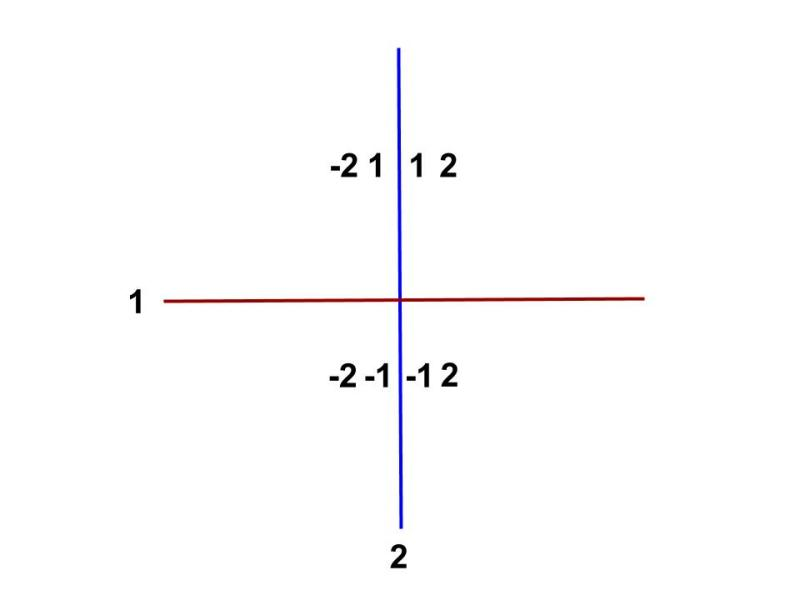
\includegraphics[width=0.85\textwidth]{ne585/mcnp_basic.surface.jpg}
%       \caption{}
    \end{figure}
\end{frame}


\section{Cells}


\addtocounter{framenumber}{-1} 
\begin{frame}{Surfaces define cells}
    \begin{enumerate}[series=outerlist,topsep=0pt,itemsep=21pt,leftmargin=*,label=(\arabic*)]
        \item[]Each has a distinct volume because they are defined by density (134-5)
        \item[]Intersection, union, of defined surfaces; NOT cell
    \end{enumerate}
    \small
    \begin{enumerate}[series=outerlist,topsep=7pt,itemsep=1pt,leftmargin=*,label=(\arabic*)]
        \item[]\texttt{100    1 -2.03                -10 11 -12                 \$metal/salt-filled cathode basket}
        \item[]\texttt{101    2 -3.58    (10:-11)    -12 -13 14                 \$MgO cathode basket}
        \item[]\texttt{102    3 -0.00178 (12:13:-14) -15 16 -17                 \$Ar content in equipment}
        \item[]\texttt{103    4 -7.92    (15:-16:17) -18 -19 20                 \$steel equipment}
        \item[]\texttt{104    3 -0.00178 (18:19:-20) -50 51 -52 53 54 -55       \$rest of SE hot cell}
        \item[]\texttt{110    3 -0.00178             -52 53 54 -55 -61 70       \$SW hot cell}
        \item[]\texttt{111    3 -0.00178              54 -55 -61 62 70 -72      \$NW hot cell}
        \item[]\texttt{112    3 -0.00178             -50 51 54 -55 62 -72       \$NE hot cell}
    \end{enumerate}
\end{frame}


\begin{frame}{Finite cylinder with equal radius and height}
    \small
    \begin{enumerate}[series=outerlist,topsep=0pt,itemsep=1pt,leftmargin=*,label=(\arabic*)]
        \item[]\texttt{10     CZ  22.23        \$metal/cathode basket radius}
        \item[]\texttt{11     PZ  100          \$metal/cathode basket above the floor}
        \item[]\texttt{12     PZ  122.23       \$metal/cathode basket height+floor height}
    \end{enumerate}
    \normalsize
    \begin{enumerate}[series=outerlist,topsep=21pt,itemsep=21pt,leftmargin=*,label=(\arabic*)]
        \item[]100 cm above the floor
    \end{enumerate}
\end{frame}


\begin{frame}{Use the union operator to assemble larger cells or get around harder shapes}
    \small
    \begin{enumerate}[series=outerlist,topsep=0pt,itemsep=1pt,leftmargin=*,label=(\arabic*)]
        \item[]\texttt{10     CZ  22.23         \$metal/cathode basket radius}
        \item[]\texttt{11     PZ  100           \$metal/cathode basket above the floor}
        \item[]\texttt{12     PZ  122.23        \$metal/cathode basket height+floor height}
        \item[]\texttt{13     CZ  27.23         \$5 cm thick MgO cathode basket}
        \item[]\texttt{14     PZ  95            \$height above the floor/cathode basket bottom}
            \vspace{0.10in}
        \item[]\texttt{100    (10:-11)  -12 -13 14   \$MgO cathode basket}
    \end{enumerate}
    \normalsize
    \begin{enumerate}[series=outerlist,topsep=19pt,itemsep=21pt,leftmargin=*,label=(\arabic*)]
        \item[]Use of \href{https://github.com/TheDoctorRAB/igem}{\texttt{NOT} cell} is actually cleaner 
    \end{enumerate}
\end{frame}


\begin{frame}{}
    \begin{figure}
        \centering
        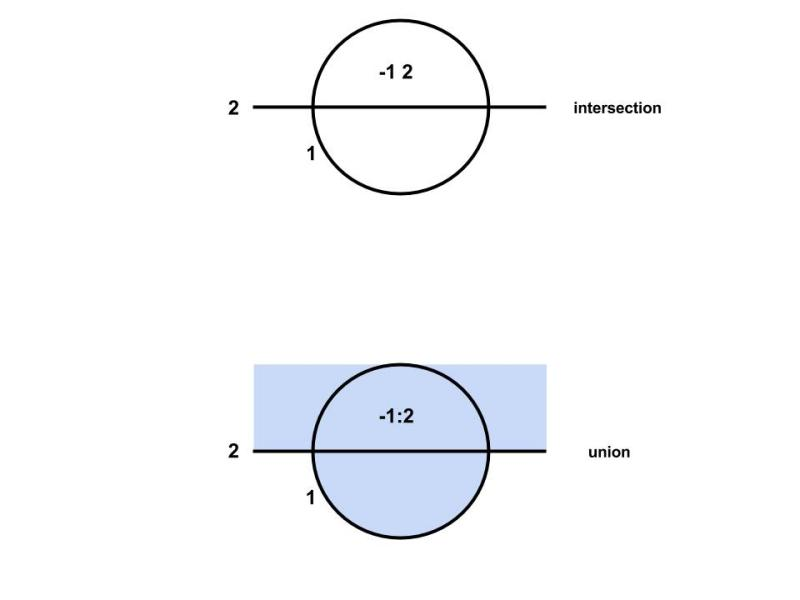
\includegraphics[width=0.85\textwidth]{ne585/mcnp_surface.union.jpg}
%       \caption{}
    \end{figure}
\end{frame}


\section{Universes}


\addtocounter{framenumber}{-1} 
\begin{frame}{\href{https://github.com/TheDoctorRAB/igem}{Universes} are useful for repeating units}
    \begin{enumerate}[series=outerlist,topsep=0pt,itemsep=21pt,leftmargin=*,label=(\arabic*)]
        \item[]Or `nested geometries' at multiple levels
        \item[]For a reactor core
        \item[]Remember `unit cells' from reactor theory?
        \item[]Group a collection of cells into a universe
        \item[]Use VisEd for help on geometries
    \end{enumerate}
\end{frame}


\begin{frame}{}
    \begin{figure}
        \centering
        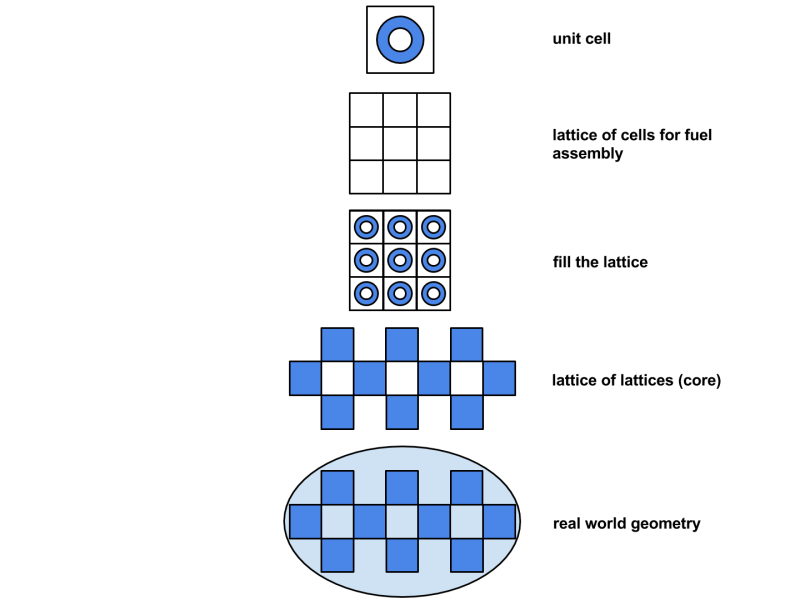
\includegraphics[width=0.80\textwidth]{ne585/mcnp_universe.jpg}
%       \caption{}
    \end{figure}
\end{frame}


\section{Other tips}


\addtocounter{framenumber}{-1} 
\begin{frame}{Other tips}
    \begin{enumerate}[series=outerlist,topsep=0pt,itemsep=21pt,leftmargin=*,label=(\arabic*)]
        \item[]Someone already has made the same error as you -- look it up
        \item[]Do not have coinciding surfaces
        \item[]Check the model space with VisEd or the plotter
        \item[]It will show where there are problems
        \item[]Use the \href{https://uidaho.pressbooks.pub/nuclearengineering/chapter/mcnp/}{compendium} in the \acs{oer} to get weight fractions of common materials
        \item[]Then look up the cross section libraries (.70c, etc.) in Appendix G
    \end{enumerate}
\end{frame}


\section{Additional information}


\addtocounter{framenumber}{-1} 
\begin{frame}{Additional information in the slides}
    \begin{enumerate}[series=outerlist,topsep=0pt,itemsep=3pt,leftmargin=*,label=(\arabic*)]
        \item[]\textbf{HTGR modeling (148-165)}
        \item[]TRISO pebbles
        \item[]Example of embedded universes
            \vspace{0.05in}
        \item[]\textbf{Collision physics (166-205)}
        \item[]How particles travel
        \item[]Interactions
        \item[]Determine which isotope the interaction is with  
        \item[]Determine which interaction type for that isotope  
        \item[]Determine the energy \& direction of the exiting particle  
        \item[]Determine if secondary particles were produced  
        \item[]Sample flight distance  
        \item[]Biasing + weight adjustments  
        \item[]Tallies of quantities of interest based on pdfs
    \end{enumerate}
\end{frame}


\section{\acs{mcp} quality control}
\section{Mean \& variance}


\addtocounter{framenumber}{-2} 
\begin{frame}{Really we only need mean and variance for most problems}
    \begin{enumerate}[series=outerlist,topsep=0pt,itemsep=21pt,leftmargin=*,label=(\arabic*)]
        \item[]For random variable $x$ of function $r(x)$ with pdf $f(x)$
    \end{enumerate}

    \vspace*{\fill}

    \begin{equation}
        \LARGE
         \mu \equiv \int r(x)f(x)dx
    \end{equation}

    \begin{equation}
        \LARGE
        \sigma^2 \equiv \int r^2(x)f(x)dx -\mu^2
    \end{equation}
\end{frame}


\begin{frame}{Monte Carlo randomly samples to get moments}
    \begin{equation}
        \LARGE
        \overline{r} \approx \frac{1}{N}\sum_{j=1}^N r(x_j)
    \end{equation}

    \begin{equation}
        \LARGE
        \sigma^2_{\overline{r}} \approx \frac{1}{N-1}(\frac{1}{N}\sum_{j=1}^N r(x_j) - \overline{r}^2)
    \end{equation}

    \vspace*{\fill}

    \begin{enumerate}[series=outerlist,topsep=0pt,itemsep=18pt,leftmargin=*,label=(\arabic*)]
        \item[]This is based on the law of large numbers  
        \item[]Sample average will approach the true expected value with increasing $N$ 
        \item[]Central limit theorem states it will take on a normal distribution (210)
        \item[]So the tally is the most probable result (basically)
    \end{enumerate}
\end{frame}


\section{Statistical checks}


\addtocounter{framenumber}{-1} 
\begin{frame}{Statistical checks are provided for each tally}
    \begin{enumerate}[series=outerlist,topsep=0pt,itemsep=5pt,leftmargin=*,label=(\arabic*)]
        \item[]Relative error ($R$) = standard deviation/mean
        \item[]$R$ should decrease with increasing sqrt $N$ smoothly
            \vspace{0.15in}
        \item[]\acs{fom} is a measure of relative error and computer time
        \item[]\acs{fom} should be roughly constant
            \vspace{0.15in}
        \item[]\acf{vov} is relative variance of $R$
        \item[]Essentially verifies the central limit theorem
        \item[]Decrease smoothly with $N$
        \item[]Explained in depth in the manual
            \vspace{0.15in}
        \item[]Statistical checks are to avoid undersampling
    \end{enumerate}
\end{frame}


\begin{frame}{More about statistical checks (2-132)}
    \begin{enumerate}[series=checks,topsep=0pt,itemsep=5pt,leftmargin=*,label=(\arabic*)]
        \item[]\textbf{Mean}
        \item A nonmonotonic behavior (no up or down trend) in the estimated mean as a function of the number histories $N$ for the last half of the problem
            \vspace{0.10in}
        \item[]\textbf{R}
        \item An acceptable magnitude of the estimated $R$ of the estimated mean (less than 0.05 for a point detector tally or less than 0.10 for a non-point detector tally)
        \item A monotonically decreasing $R$ as a function of the number histories $N$ for the last half of the problem
        \item $N^{0.5}$ decrease in the $R$ as a function of $N$ for the last half of the problem
            \vspace{0.10in}
        \item[]\textbf{\acs{vov}}
        \item The magnitude of the estimated \acs{vov} should be less than 0.10 for all types of tallies
        \item A monotonically decreasing \acs{vov} as a function of $N$ for the last half of the problem
        \item A $\frac{1}{N}$ decrease in the \acs{vov} as a function of $N$ for the last half of the problem
    \end{enumerate}
\end{frame}


\begin{frame}[t]{}
    \begin{enumerate}[resume=checks,topsep=0pt,itemsep=5pt,leftmargin=*,label=(\arabic*)]
        \item[]\textbf{\acs{fom}}
        \item A statistically constant value of \acs{fom} as a function of $N$ for the last half of the problem
        \item A nonmonotonic behavior in \acs{fom} as a function of $N$ for the last half of the problem
        \item[] $FOM \equiv \frac{1}{R^2 T}$
            \vspace{0.10in}
        \item[]\textbf{f(x)}
        \item The SLOPE (see page 2–127 Pareto fit) of the 25 to 201 largest positive (negative with a negative DBCN(16) entry) history scores $x$ should be greater than 3.0 so that the second moment will exist if the SLOPE is extrapolated to infinity
    \end{enumerate}
\end{frame}


\section{Criticality}


\addtocounter{framenumber}{-1} 
\begin{frame}{For criticality, a little different (247)}
    \begin{enumerate}[series=outerlist,topsep=0pt,itemsep=5pt,leftmargin=*,label=(\arabic*)]
        \item[]Assume an initial $k$ ($k = 1$, just use default \texttt{KCODE}; \texttt{KSRC = x y z} for a point in the middle of the source)  
        \item[]Fission sites are sampled from the initial source distribution
        \item[]Follow a `batch' of histories to estimate $k$ (collectively called cycles)
        \item[]When they converge, discard the tallies
        \item[]Then start the new iterations until variances decrease
        \item[]The idea is to run from 1 to N+D cycles (D = discard number) to converge the initial guess
        \item[]Then run for $N$ cycles to get a confident $k$
        \item[]The gist is when obtaining $k$, the value is statistically robust
        \item[]Typically, just start with the \acs{mcp} defaults and that should be good enough
        \item[]Having some reasonable idea of the theory can help with higher level problems
    \end{enumerate}
\end{frame}


\section{Variance reduction}


\addtocounter{framenumber}{-1} 
\begin{frame}{\acs{mcp} also comes with many many variance reduction techniques (310)}
    \begin{enumerate}[series=checks,topsep=0pt,itemsep=5pt,leftmargin=*,label=(\arabic*)]
        \item[]Increase $N$ for the first move (or cycles)
            \vspace{0.10in}
        \item[]\textbf{Modified sampling}
        \item[]Modify the pdfs for physics interactions to favor events/tallies of interest
            \vspace{0.10in}
        \item[]\textbf{Population control}
        \item[]Use splitting/roulette to increase particles in certain geometric regions
        \item[]Control number of samples taken in specified regions of the phase space
        \item[]\acf{wwg} and importance functions
            \vspace{0.10in}
        \item[]\textbf{Truncation}
        \item[]Kill particles in uninteresting parts of problem
        \item[]May be necessary in order to sample rare events
        \item[]More samples (with less weight each) $\rightarrow$ smaller variance in tallies
    \end{enumerate}
\end{frame}


\begin{frame}[t]{}
    \begin{enumerate}[series=checks,topsep=0pt,itemsep=5pt,leftmargin=*,label=(\arabic*)]
        \item[]\textbf{Deterministic methods}
        \item[]Replace portions of a particle random walk by the expected results obtained from a deterministic calculation
        \item[]
            \vspace{0.20in}
        \item[]Not a huge problem with basic criticality problems
    \end{enumerate}
\end{frame}


\begin{frame}{There are cards to do this so you don't have to actually code}
    \begin{equation}
        \LARGE
        \mu = \int r(x)\frac{f(x)}{g(x)}g(x)dx
    \end{equation}

    \vspace*{\fill}

    \begin{equation}
        \LARGE
        \sigma^2 = [r(x)\frac{f(x)}{g(x)}]^2g^2(x)dx - \mu^2
    \end{equation}

    \vspace*{\fill}

    \begin{enumerate}[series=outerlist,topsep=0pt,itemsep=21pt,leftmargin=*,label=(\arabic*)]
        \item[]Choose $g(x)$ to reduce variance; e.g., $R$, \acs{vov}
        \item[]Favor directions more important to tallies
        \item[]Change weights, importance, bias pdfs, and so much more
        \item[]It isn't a science and comes with experience
    \end{enumerate}
\end{frame}


\begin{frame}{Different problems have different approaches}
    \begin{enumerate}[series=techniques,topsep=0pt,itemsep=3pt,leftmargin=*,label=(\arabic*)]
        \item Time and energy cutoffs
        \item Geometry splitting \& roulette
        \item \acsp{wwg}
        \item Exponential transform
        \item Forced collisions
        \item Energy splitting \& roulette
        \item Time splitting \& roulette
        \item Point and ring detectors
        \item DXTRAN
        \item Implicit capture
        \item Weight cutoff
        \item General source biasing
        \item Secondary particle biasing
        \item Bremsstrahlung energy biasing
    \end{enumerate}
\end{frame}


\section{Keep the manual handy}


\addtocounter{framenumber}{-1} 
\begin{frame}{Jezebel example}
    \begin{enumerate}[series=techniques,topsep=0pt,itemsep=21pt,leftmargin=*,label=(\arabic*)]
        \item[]\href{https://github.com/TheDoctorRAB/mcnpx.decks/blob/master/criticality/jezebel.inp}{Deck on GitHub}
        \item[]Set up examples with radii
        \item[]\href{https://www.osti.gov/servlets/purl/10171566}{Criticality guide}
    \end{enumerate}
\end{frame}


\begin{frame}[plain]{}
    \begin{figure}
        \centering
        \includegraphics[width=0.75\textwidth]{ne585/5-final.jpg}
%        \caption{}
    \end{figure}
\end{frame}


%%%%%%%
%\begin{frame}{}
%    \begin{columns}
%
%        \begin{column}{0.50\textwidth}
%            \begin{enumerate}[series=outerlist,topsep=0pt,itemsep=21pt,leftmargin=*,label=(\arabic*)]
%                \item[]
%                \item[]
%            \end{enumerate}
%        \end{column}
%
%        \begin{column}{0.50\textwidth}
%            \begin{enumerate}[series=outerlist,topsep=0pt,itemsep=21pt,leftmargin=*,label=(\arabic*)]
%                \item[]
%                \item[]
%            \end{enumerate}
%        \end{column}
%
%    \end{columns}
%\end{frame}

%    \begin{figure}
%        \centering
%        \includegraphics[width=0.75\textwidth]{wsc.png}
%        \caption{\acs{wsc}}
%    \end{figure}


%\begin{frame}{References}
%    \bibliographystyle{nsf}
%    \footnotesize
%    \bibliography{references}
%\end{frame}
%%%%%%%


\end{document}
